\documentclass[12pt,letterpaper]{article}
\usepackage[utf8]{vietnam}
\usepackage{fullpage}
\usepackage[top=2cm, bottom=4.5cm, left=2.5cm, right=2.5cm]{geometry}
\usepackage{amsmath,amsthm,amsfonts,amssymb,amscd}
\usepackage{lastpage}
\usepackage{enumerate}
\usepackage{fancyhdr}
\usepackage{mathrsfs}
\usepackage{xcolor}
\usepackage{graphicx}
\usepackage{listings}
\usepackage{hyperref}
\usepackage[demo]{graphicx}
\usepackage{caption}
\usepackage{subcaption}
\hypersetup{%
  colorlinks=true,
  linkcolor=blue,
  linkbordercolor={0 0 1}
}
 
\renewcommand\lstlistingname{Algorithm}
\renewcommand\lstlistlistingname{Algorithms}
\def\lstlistingautorefname{Alg.}

\lstdefinestyle{Python}{
    language        = Python,
    frame           = lines, 
    basicstyle      = \footnotesize,
    keywordstyle    = \color{blue},
    stringstyle     = \color{green},
    commentstyle    = \color{red}\ttfamily
}

\setlength{\parindent}{0.0in}
\setlength{\parskip}{0.05in}

% Edit these as appropriate
\newcommand\course{Massp2019}
\newcommand\hwnumber{PCA Report}                  % <-- homework number
\newcommand\NetIDa{Nguyen Quang Huy}           % <-- NetID of person #1

\pagestyle{fancyplain}
\headheight 35pt
\lhead{\NetIDa}
%\lhead{\NetIDa\\\NetIDb}                 % <-- Comment this line out for problem sets (make sure you are person #1)
\chead{\textbf{\Large Hw \hwnumber}}
\rhead{\course \\ \today}
\lfoot{}
\cfoot{}
\rfoot{\small\thepage}
\headsep 1.5em


\begin{document}
\section*{Principal Component Analysis là gì}

Principal Component Analysis là phương pháp dùng để giảm số chiều của dữ liệu bằng cách tìm các chiều là thành phần chính của dữ liệu, từ đó ta có thể biểu diễn dữ liệu theo công thức:
$$
    X = X_0 + z_1*X_1 + z_2*X_2 + ... + z_k*X_k    \quad (1)
$$
Với 
\begin{enumerate}
    \item k là số chiều của dữ diệu
    \item $X_0$ là means của training data
    \item $X_i$ là basic function
    \item $z_i$ là toạ độ của điểm dữ liệu
\end{enumerate}
Dữ liệu qua thuật toán PCA trở thành các điểm toạ độ có thể sử dụng để so sánh hay lưu trữ...

\section*{Encode}
Khi áp dụng thuật toán ta có U là ma trận lưu basic functions, từ đó có thể tích toạ độ z của điểm dữ liệu bằng cách chiếu điểm dữ liệu lên các trục số
$z = U^T * x$ với $x = X - X_0$
\section*{Decode}
Với z là toạ độ của điểm dữ liệu, khi decode dữ liệu ta chỉ cần thay toạ độ của dữ liệu vào công thức (1)
\section*{Thực nghiệm trên code}
Áp dụng với bài toán encode và decode T ảnh
Với mỗi K thuộc [1,10,20,50,100], ta có ảnh decode như sau: 

\begin{figure}
\captionsetup[subfigure]{labelformat=empty}
\centering
\begin{subfigure}{.5\textwidth}
  \centering
  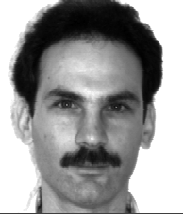
\includegraphics[width=.4\linewidth]{ori02.png}
  \caption{origin picture}
  \label{fig:sub1}
\end{subfigure}%
\begin{subfigure}{.5\textwidth}
  \centering
  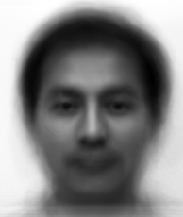
\includegraphics[width=.4\linewidth]{res021.png}
  \caption{K = 1, loss = 33404.46579972785}
  \label{fig:sub2}
\end{subfigure}
\label{fig:test}
\end{figure}


\begin{figure}
\captionsetup[subfigure]{labelformat=empty}
\centering
\begin{subfigure}{.5\textwidth}
  \centering
  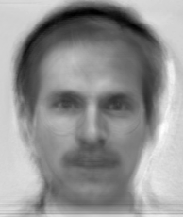
\includegraphics[width=.4\linewidth]{res0210.png}
  \caption{K = 10, loss = 31214.950574420687}
  \label{fig:sub1}
\end{subfigure}%
\begin{subfigure}{.5\textwidth}
  \centering
  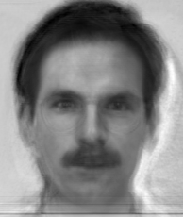
\includegraphics[width=.4\linewidth]{res0220.png}
  \caption{K = 20, loss = 30860.068222190162}
  \label{fig:sub2}
\end{subfigure}
\label{fig:test}
\end{figure}


\begin{figure}
\captionsetup[subfigure]{labelformat=empty}
\centering
\begin{subfigure}{.5\textwidth}
  \centering
  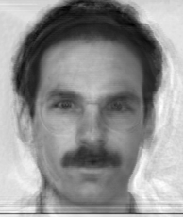
\includegraphics[width=.4\linewidth]{res0250.png}
  \caption{K = 50, loss = 30534.718245444663}
  \label{fig:sub3}
\end{subfigure}%
\begin{subfigure}{.5\textwidth}
  \centering
  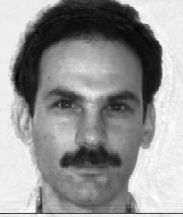
\includegraphics[width=.4\linewidth]{res02100.png}
  \caption{K = 100, loss = 30305.81835208503}
  \label{fig:sub4}
\end{subfigure}
\label{fig:test}
\end{figure}

\centering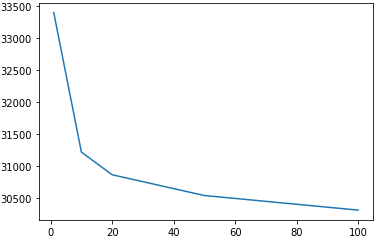
\includegraphics[scale=1]{graph.png}
\\ reconstruction errors
\section*{Quiz}
\begin{enumerate}
    \item coordinate vector $z = U'.dot(x)$ với $ x = im - mean $ 
    \\ Ta có: 
    $x = z_1*X_1 + z_2*X_2 + ... + z_k*X_k$
    \\ Vì các basic vector vuông góc với nhau nên khi nhân 2 ma trận ta sẽ chiếu được giá trị của điểm lên các trục
    \item tính compression ratio cho ví dụ eigenface hôm nay nếu chỉ truyền 1 coordinate vector length-100 cho mỗi hình
    \\ dung lượng phải lưu cho T hình gốc là ma trận H*W*T (trong đó H và W là kích thước 1 hình
    \\ dung lượng phải lưu cho T hình đã nén là K ma trận basis vector có kích thước H*W*K và K vector coordinate có kích thước K*T
    \\ vậy tỉ lệ nén với K = 100 khi nén T hình là 
    $$ 
        \frac{H*W*100 + T*100}{H*W*T}
    $$
\end{enumerate}
\end{document}
